% Compiles with IEEEtran (e.g. on Overleaf). If IEEEtran.cls is not installed,
% it falls back to a two-column article with IEEE-like margins and headings.
\IfFileExists{IEEEtran.cls}{%
  \documentclass[conference]{IEEEtran}
  \newif\ifieee\ieeetrue
}{%
  \documentclass[10pt,twocolumn,letterpaper]{article}
  \newif\ifieee\ieeefalse
}
\ifieee\else
  \usepackage[top=0.75in,bottom=1in,left=0.625in,right=0.625in,columnsep=0.25in]{geometry}
  \usepackage{mathptmx}
  \usepackage[T1]{fontenc}
  \usepackage{titlesec}
  \renewcommand{\thesection}{\Roman{section}}
  \renewcommand{\thesubsection}{\Alph{subsection}}
  \titleformat{\section}{\centering\normalsize\scshape}{\thesection.}{0.5em}{}
  \titleformat{\subsection}{\normalsize\itshape}{\thesubsection.}{0.5em}{}
  \titlespacing*{\section}{0pt}{8pt}{4pt}
  \titlespacing*{\subsection}{0pt}{6pt}{3pt}
  \usepackage[font=footnotesize,labelsep=period]{caption}
  \newcommand{\IEEEauthorblockN}[1]{{\large #1}\\}
  \newcommand{\IEEEauthorblockA}[1]{\normalsize\itshape\begin{tabular}{@{}c@{}}#1\end{tabular}}
  \newenvironment{IEEEkeywords}{\par\noindent\textbf{\textit{Index Terms}---}\itshape}{\par}
  \renewenvironment{abstract}{\par\noindent\textbf{\textit{Abstract}---}\bfseries}{\par\medskip}
  \pagestyle{plain}
\fi
\usepackage{amsmath}
\usepackage{graphicx}
\usepackage{booktabs}
\usepackage{cite}
\usepackage{url}
\graphicspath{{../figures/}}

\begin{document}

\title{Midnight, Not Midday: Air Conditioning, Electric Scooter Charging and Distribution Transformer Ageing in a Lahore Neighbourhood}

\author{\IEEEauthorblockN{Syeda Tehreem Gillani}
\IEEEauthorblockA{Department of Computer Science, FAST National University of Computer and Emerging Sciences, Karachi, Pakistan}}

\maketitle

\begin{abstract}
Pakistan plans to put about two million electric two-wheelers on the road by
2030, and most will be charged at home, on distribution transformers that
already carry heavy air-conditioning load in summer. The studies of charging and
transformer ageing reviewed here deal with cars in the United States, Europe
and Australia, and the common advice to charge ``at night, off peak'' assumes
that household load falls at night. This study tests that assumption with one
year of measured one-minute household data from Lahore (PRECON). Every house
uses more power as the day gets hotter (median 77~W per kelvin of daily mean
temperature above about 22.5\,$^\circ$C, tested on unseen weeks), and a
virtual feeder of 34 houses peaks around midnight from April to September, not
in the afternoon. Scooter charging from two use profiles is added under five
charging rules, and the transformer's hot-spot temperature and insulation
ageing are computed with the IEC 60076-7 thermal model. With a scooter in
every house (4\,\% more energy), charging on arrival raises yearly ageing by
21\,\%; a timer that starts charging when the tariff peak window ends raises
it by 36\,\%, because it lands on the night peak; a timer that finishes
charging just before the morning departure raises it by 8\,\%, the same as an
ideal valley-filling schedule. On a tighter transformer the same rules give
$+50$\,\%, $+110$\,\% and $+11$\,\%. A climate 2\,K warmer, applied through the
measured temperature slope, raises baseline ageing 2.4 times, more than any
charging rule.
\end{abstract}

\begin{IEEEkeywords}
distribution transformer, electric two-wheeler, smart charging, air conditioning, PRECON, IEC 60076-7, Pakistan
\end{IEEEkeywords}

\section{Introduction}
Pakistan's National Electric Vehicle Policy 2025--30 counts about 2.05 million
two-wheelers in its target of 2.21 million new energy vehicles \cite{saarc2026}.
E-scooters sold locally have small packs and chargers (the Eveon Pronto, for
example, has a 72~V, 32~Ah pack and a 4~A charger \cite{pronto}), so they are
charged from ordinary house sockets. Their load therefore lands on the same
11/0.4~kV distribution transformers that serve residential air conditioning
(AC), which drives the summer load in the data used here (Section~VI-A).

The insulation of an oil-immersed transformer ages with its hot-spot
temperature, which depends on the load, the ambient temperature and the
timing of both \cite{iec60076}. A charging rule that moves load in time can
therefore change ageing even when it adds no energy. This has been studied in
detail for electric cars (Section~II), and the usual conclusion is that
uncontrolled evening charging raises ageing and that moving it later helps.
Two things make the Pakistani case different: the vehicles are small
two-wheelers with sub-kilowatt chargers, and summer nights in Lahore are hot,
so household AC may keep the night load high.

This paper asks two questions. When is a Lahore neighbourhood transformer
most loaded, according to measured household data? And for the same scooter
energy, how much does the time of charging change the transformer's yearly
ageing? It uses PRECON \cite{precon}, one year of one-minute power data from
houses in Lahore, with NASA POWER weather \cite{nasapower}, and extends two
earlier studies by the author: a home PV and battery schedule for Karachi
\cite{gillaniA} and a thermal-cycling study of scooter motor controllers
\cite{gillani2}, whose scooter model supplies the charging energy here.

Section~II reviews related work and Section~III states the gap and the
contributions. Sections~IV and~V give the data and the models,
Section~VI the results, and Section~VII the limitations.

\section{Related Work}
\subsection{EV charging and distribution transformer ageing}
Gong \emph{et al.} \cite{gong2012} combined a dynamic thermal model of a
residential distribution transformer with Monte Carlo charging scenarios to
estimate how plug-in vehicle charging affects transformer life. Hilshey \emph{et al.} \cite{hilshey2013} used the IEEE C57.91
model for a 25~kVA transformer serving 12 homes and compared a cool climate
(Burlington, Vermont) with a hot one (Phoenix, Arizona). Uncontrolled Level~2
charging raised ageing by a factor of 9.79 in Phoenix against 2.34 in
Burlington, so the ambient temperature mattered as much as the charging
itself. They also found that simply delaying Level~2 charging until after
midnight increased ageing, and that a smart charging scheme that used the transformer temperature reduced
ageing by a factor of 4.8 to 6.3. Soleimani and Kezunovic \cite{soleimani2020}
used the same IEEE model with Nissan LEAF and Bolt charging at 40\,\%
penetration and proposed a fuzzy-logic smart charging scheme to limit loss of
life. Clement-Nyns \emph{et al.} \cite{clementnyns2010} looked at a Belgian
residential grid with Belgian residential load profiles; uncoordinated evening charging
gave the worst voltage deviations, and at 30\,\% penetration their test feeder
needed a larger transformer.

Rooftop PV interacts with these results. Geiles and Islam \cite{geiles2013}
found that rooftop PV can offset part of the ageing caused by vehicle
charging. Behi \emph{et al.} \cite{behi2017} applied the IEC thermal model to
a 200~kVA transformer on a Perth feeder; PV lowered loss of life by about
58\,\% by relieving off-peak loading, but did not reduce the peak, because the
peak and PV output did not coincide, and PV with demand response together cut
loss of life by about 90\,\%.

\subsection{Timing of home charging}
At a larger scale, Muratori \cite{muratori2018} showed that uncoordinated home
charging reshapes residential demand and that clustering of vehicles raises
local peaks. Powell \emph{et al.}
\cite{powell2022} found that more daytime charging reduces grid impacts, and
that home charging scheduled locally to off-peak hours can itself create new
peaks. Li and Jenn \cite{lijenn2024} modelled California's distribution
networks and found that about half of the feeders would need upgrades by 2035
under uncontrolled charging, with residential feeders needing about twice the
upgrades of commercial ones and residential overloads occurring at night. A
recurring message across these studies is that a timer that sends every
vehicle to the same ``off-peak'' hour can move the problem rather than solve
it.

\subsection{Temperature and household demand}
Auffhammer \emph{et al.} \cite{auffhammer2017} showed for the United States
that peak electricity demand is more sensitive to temperature than average
demand, so warming matters most at the peak. Change-point regression, in
which load is flat below a balance temperature and rises linearly above it,
is a standard way to measure such sensitivity from metered data
\cite{kissock2003}.

For Pakistan, PRECON \cite{precon} is the main open source of high-resolution
household data. Its authors later used ambient temperature as an input for
short-term load forecasting on the same data, where regression and support
vector models did better than a neural network, and noted load shedding in
the records \cite{nadeem2020}. Bajwa \emph{et al.} \cite{bajwa2026} used
PRECON within a nine-city climate study and found that AC takes a mean
21.4\,\% of household electricity, rising above 33\,\% in June and July; their
household analysis reports monthly shares and does not model load against
temperature, time of day, or the network.

\subsection{Electric two-wheelers}
Abdul-Manan \emph{et al.} \cite{abdulmanan2022} found that in India electric
two-wheelers already reduce life-cycle greenhouse gas emissions compared with
petrol ones and recommended prioritising them, noting that their small,
removable batteries can be charged indoors or swapped. Corti \emph{et al.}
\cite{corti2024} reviewed charging infrastructure for electric micromobility
and noted its lower power and the lack of a standard output voltage. Huu and
Ngoc \cite{huu2021} proposed a load-profile tracking algorithm for
two-wheeler charging stations with PV in Vietnam, aimed at filling valleys
and cutting peaks. Table~\ref{tab:lit} summarises the studies closest to this
one.

\begin{table}[t]
\centering
\caption{Studies closest to this work}
\label{tab:lit}
\footnotesize
\begin{tabular}{@{}p{0.2\columnwidth}p{0.17\columnwidth}p{0.53\columnwidth}@{}}
\toprule
Study & Vehicles & What it shows \\
\midrule
Gong \cite{gong2012} & cars & dynamic thermal model with Monte Carlo charging \\
Hilshey \cite{hilshey2013} & cars & hot climate ageing ${\approx}4\times$ cool; after-midnight delay can raise ageing \\
Soleimani \cite{soleimani2020} & cars & fuzzy smart charging to limit loss of life \\
Behi \cite{behi2017} & none (PV, DR) & IEC model; PV helps off-peak, not the peak \\
Li, Jenn \cite{lijenn2024} & cars & half of feeders need upgrades by 2035; residential overloads at night \\
Huu, Ngoc \cite{huu2021} & two-wheelers & station scheduling with PV; no transformer ageing \\
Bajwa \cite{bajwa2026} & none & PRECON AC share by month; no network \\
This work & two-wheelers & measured 1-min Lahore load, IEC ageing, Pakistani tariff timer \\
\bottomrule
\end{tabular}
\end{table}

\section{Research Gap and Contributions}
From the studies above, three gaps stand out.
\begin{enumerate}
\item Transformer-ageing studies of home charging that were found deal with
cars with charging power of several kilowatts, in the United States, Europe
and Australia. The two-wheeler studies found deal with emissions, charger
design or charging stations, not with the residential transformer.
\item The advice to charge at night assumes a night valley in household
load. Hilshey \emph{et al.} \cite{hilshey2013} and Li and Jenn \cite{lijenn2024}
already show that night charging can overload US transformers, but no study
found here checks the shape of the night load in a hot South Asian city with
measured data. Work on PRECON so far forecasts load or reports AC shares
\cite{nadeem2020,bajwa2026}; it does not ask when a shared transformer is most
loaded.
\item No study found evaluates a timer tied to Pakistan's time-of-use peak
windows \cite{nepra2026} against transformer ageing.
\end{enumerate}

This paper makes four contributions. (i) It measures the temperature
sensitivity of 41 PRECON houses and of a 34-house virtual feeder, with a test
on held-out weeks. (ii) It shows that this feeder peaks near midnight in
summer and that the summer tariff peak window ends just as the feeder's own
peak begins. (iii) It compares five charging rules, including the UK default
random delay and a NEPRA-window timer, by IEC 60076-7 insulation ageing, and
shows that the rule matters more than the energy. (iv) The code, derived data
and an interactive tool are open, so every number can be reproduced.

\section{Data}
\subsection{Household data}
PRECON gives one-minute kW for each house from June 2018 to May 2019, with a
total-load column and, in 33 houses, one or more metered AC circuits
\cite{precon}. House~35 was not in the downloaded archive, so 41 houses are
used. The files contain no missing minutes, although the dataset paper states
that the meters switch off during power cuts \cite{precon}; the gaps were
therefore filled in some way the paper does not describe. Stretches of
10~minutes or more in which all columns of a house lie on one exact straight
line were treated as filled and removed from every fit. They are
0.4--29\,\% of a house's minutes (median 1.6\,\%). Whether they are power
cuts, logger outages or both cannot be told from the data, so no outage
analysis is attempted.

\subsection{Weather}
Hourly 2~m air temperature and global horizontal irradiance for Lahore
(31.52\,N, 74.36\,E) come from NASA POWER \cite{nasapower}, in local solar
time. POWER defines local solar time in 15$^\circ$ bands, so at this longitude
it equals Pakistan Standard Time. Each hourly value is the mean over the hour
that begins at its time stamp, so it is placed at mid-hour before linear
interpolation to minutes. The file has no missing values; the hottest hour
was 47.5\,$^\circ$C (May 2019).

\section{Methods}
\subsection{Temperature sensitivity}
For each house, daily mean load $P$ is fitted against daily mean temperature
$T$ with the change-point model \cite{kissock2003}
\begin{equation}
P = a + b\,\max(0,\;T - T_b),
\end{equation}
with $T_b$ searched on a 0.5~K grid and $a$, $b$ found by least squares. Days
need at least 20 valid hours. The model is fitted on even ISO weeks and tested
on odd weeks; the reference for the test $R^2$ is the house's mean load.

\subsection{Virtual feeder}
The 41 houses are spread over Lahore and are not on one transformer. As the
study's main assumption, houses are summed minute by minute as if they were.
Filled minutes are replaced by the same house's mean for that month and clock
hour, which models the feeder as if there were no load shedding. Seven houses
with any month less than half measured are left out of the feeder (they stay
in the temperature fits), leaving 34 houses and 1.7\,\% imputed energy. The
feeder load is converted to apparent power with an assumed power factor of
0.95.

\subsection{Scooter charging}
The scooter is the 102~kg, 72~V model of \cite{gillani2}, driving part~1 of
the WMTC cycle with the road load of UN GTR No.~2 and an assumed motor and
controller efficiency of 0.88. It needs 21.3~Wh/km at the battery; as a rough
check, the Pronto's pack and claimed 90~km range give about 26~Wh/km
\cite{pronto}. With an assumed charger efficiency of 0.85, a commuter
(24~km/day, Monday to Saturday) needs 0.60~kWh/day from the grid and a
delivery rider (96~km/day, every day) 2.41~kWh/day. The base case has one
scooter per house, 20\,\% of them delivery riders, and 0.5~kW chargers. The
Pronto's 4~A charger at a 72~V pack is about 0.3~kW at the pack, or about
0.35~kW from the grid, so 0.35~kW and 1~kW are tested as well. Commuters plug
in between 18:00 and 19:30 and leave at 07:45; delivery riders plug in
between 22:30 and 23:30 and leave at 10:45 (uniform random times). Every
scooter must get back that day's energy before it leaves. Five charging rules
are compared:
\begin{itemize}
\item \emph{plug-in}: charge at full power on arrival;
\item \emph{random delay}: as plug-in, after a random delay of up to 600~s,
the default in the UK's smart charge point rules \cite{ukscp};
\item \emph{after peak}: start when the time-of-use peak window ends. NEPRA's
LESCO tariff sets the windows as 17:00--21:00 (December--February),
18:00--22:00 (March--May and September--November) and 19:00--23:00
(June--August) \cite{nepra2026};
\item \emph{latest}: start so that charging ends exactly at departure;
\item \emph{valley fill}: charge in the lowest-load minutes before departure,
knowing the feeder load in advance. This minimises load, not ageing, and is
an ideal reference rather than a practical rule.
\end{itemize}

\subsection{Transformer thermal model}
The top-oil temperature $\theta_o$ and hot-spot temperature $\theta_h$ follow
the difference equations of IEC 60076-7, Annex C \cite{iec60076}, with load
factor $K$ (apparent power over rating) and ambient $\theta_a$:
\begin{align}
D\theta_o &= \frac{Dt}{k_{11}\tau_o}\left[\left(\frac{1+K^2R}{1+R}\right)^{x}\Delta\theta_{or} - (\theta_o-\theta_a)\right],\\
D\Delta\theta_{h1} &= \frac{Dt}{k_{22}\tau_w}\left[k_{21}\Delta\theta_{hr}K^{y} - \Delta\theta_{h1}\right],\\
D\Delta\theta_{h2} &= \frac{Dt}{\tau_o/k_{22}}\left[(k_{21}-1)\Delta\theta_{hr}K^{y} - \Delta\theta_{h2}\right],\\
\theta_h &= \theta_o + \Delta\theta_{h1} - \Delta\theta_{h2}.
\end{align}
The values are those given for ONAN distribution transformers
\cite{iec60076,is2026}: $x=0.8$, $y=1.6$, $k_{11}=1$, $k_{21}=1$, $k_{22}=2$,
$\tau_o=180$~min, $\tau_w=4$~min, $R=5$, $\Delta\theta_{or}=55$~K and
$\Delta\theta_{hr}=23$~K. The step $Dt$ is 1~min, below half the smallest
time constant as the standard requires, and the first two days are run twice
as a warm-up. Air temperature is the ambient. Ageing uses the relative ageing
rate for non-upgraded paper,
\begin{equation}
V = 2^{(\theta_h - 98)/6},
\end{equation}
summed to equivalent hours at 98\,$^\circ$C per year \cite{iec60076}. The base
rating is 100~kVA, with 75 and 200~kVA as alternatives; how many such houses
a real 100~kVA unit serves is not known here, so results are given relative
to a no-scooter run on the same rating.

\subsection{Scenarios}
Study A runs the feeder without scooters on the three ratings. Study B raises
the share of houses with a scooter from 0 to 100\,\% in steps of 25\,\%.
Study C repeats the full-adoption case for other ratings, charger powers,
1.5 times the energy, only commuters, half delivery riders, rooftop PV on
30\,\% of houses (3~kWp each from horizontal irradiance with a
performance ratio of 0.8, an assumption) and
another random seed. Study D adds 2~K to the air temperature and, on days
above the balance temperature, adds load through the measured feeder slope,
spread over the day in proportion to that day's load.

\section{Results}
\subsection{Heat and household load}
Across 41 houses the median slope is 77~W/K (interquartile range 44--120~W/K)
above a median balance temperature of 22.5\,$^\circ$C. On the unseen test
weeks the median $R^2$ is 0.68 and the median absolute error halves, from
0.39~kW without temperature to 0.19~kW. The metered AC circuits alone give a
median 38~W/K ($R^2$ 0.45), about half of the total, because not every AC unit
in a house is on a metered circuit. For the 34-house feeder the slope is
2.8~kW/K above 23\,$^\circ$C, with a test $R^2$ of 0.84 (Fig.~\ref{fig:temp}).

\begin{figure}[t]
\centering
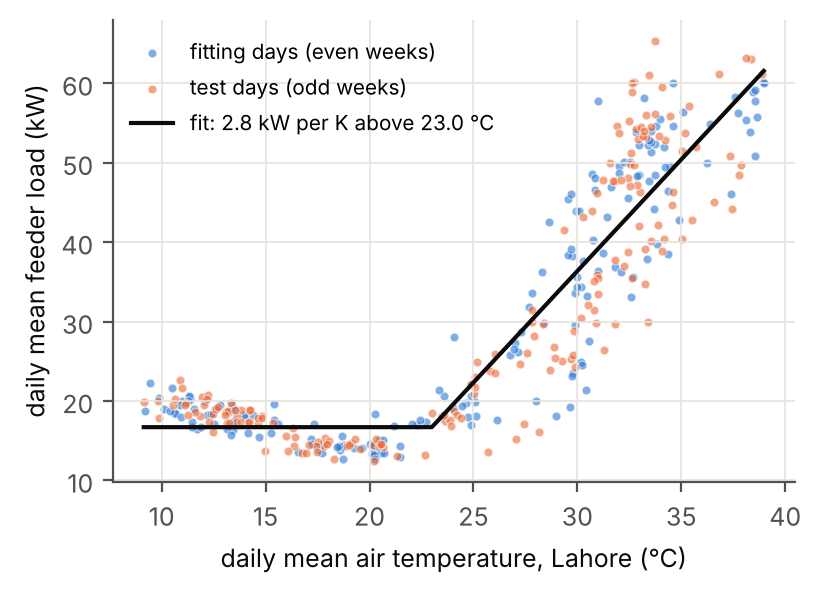
\includegraphics[width=0.66\columnwidth]{f2_temperature.png}
\caption{Daily mean feeder load against daily mean air temperature, 34 houses,
June 2018 to May 2019. The change-point fit uses even weeks only.}
\label{fig:temp}
\end{figure}

\subsection{When the feeder is most loaded}
The feeder uses 266~MWh a year. Its highest one-minute load, 101~kW, came at
23:50 on 4~June 2018, and from April to September the hour with the highest
mean load is 23:00 or midnight (Fig.~\ref{fig:shape}). From June to September
the mean load is 66~kW at midnight and falls to a minimum of 36~kW at 10:00,
while the afternoon, the hottest part of the day, sits in between. In winter
the peak moves to 19:00--20:00 and the minimum to 04:00. The summer tariff
peak window (19:00--23:00) therefore ends just as the feeder's own peak
begins. This is the household version of the night overloads that Li and
Jenn \cite{lijenn2024} found for car charging, but here it is present before
any vehicle is added.

\begin{figure}[t]
\centering
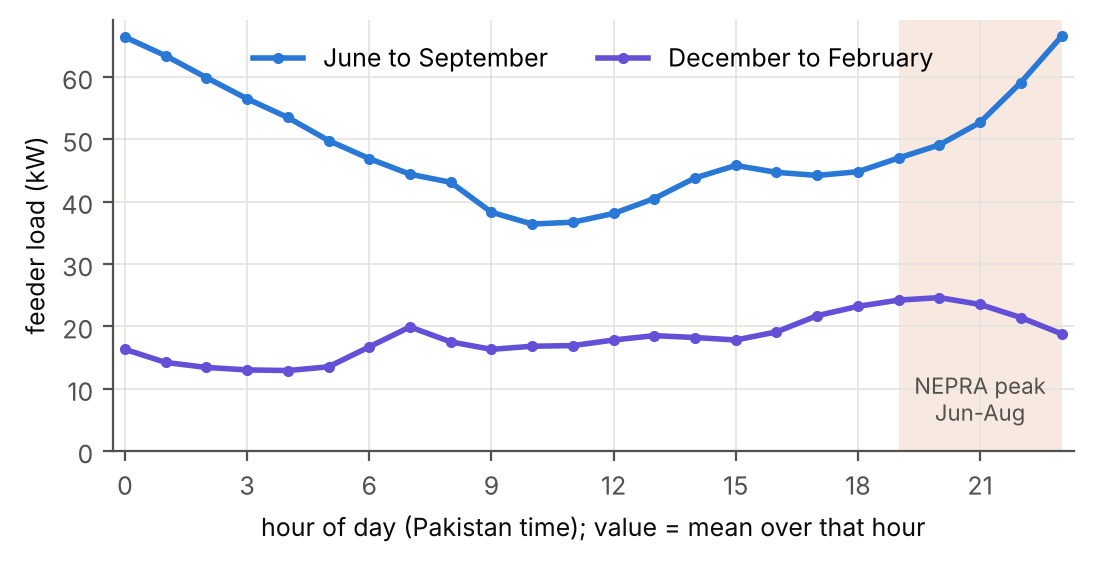
\includegraphics[width=0.86\columnwidth]{f1_daily_shape.png}
\caption{Mean feeder load by hour of day in summer and winter. Shaded: the
June--August time-of-use peak window \cite{nepra2026}.}
\label{fig:shape}
\end{figure}

\subsection{Baseline transformer ageing}
On 100~kVA the baseline peak is 1.06 per unit, the load exceeds rating for
1.7~h in the year, and the hot spot reaches 102.6\,$^\circ$C, below the
120\,$^\circ$C limit for normal cyclic loading \cite{iec60076}. Yearly ageing
is 200 equivalent hours, 90\,\% of it from June to September. On 75~kVA, which
is the same as about 45 such houses on 100~kVA, ageing is 2528~h and the hot
spot exceeds 120\,$^\circ$C on 16 days (23.2~h). On 200~kVA it is 26~h. The
rating assumption thus changes absolute ageing by two orders of magnitude,
which is why the results below are relative.

\subsection{Charging rules}
A scooter in every house adds 11.3~MWh a year, 4\,\% of the feeder's energy.
Fig.~\ref{fig:week} shows the effect during the hottest days, and
Fig.~\ref{fig:adopt} and Table~\ref{tab:rules} the yearly result.

\begin{figure}[t]
\centering
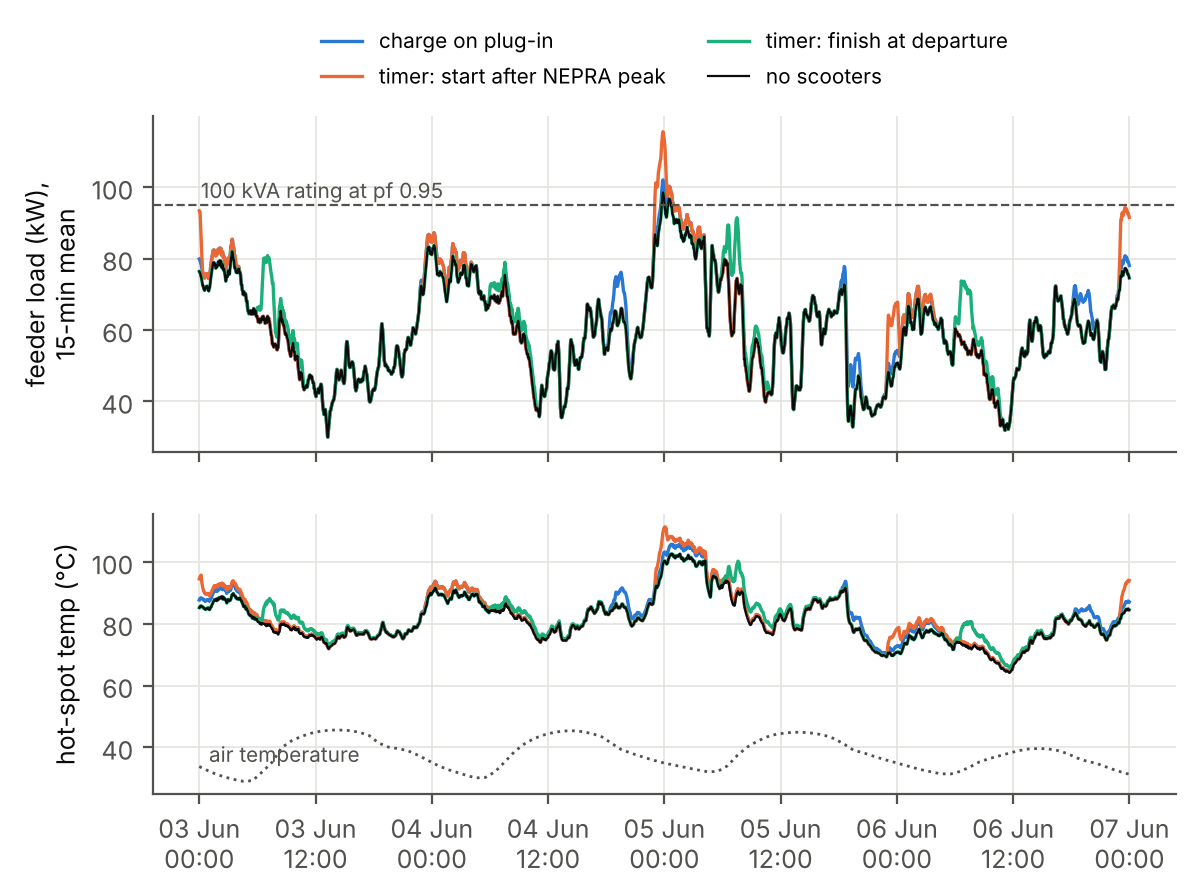
\includegraphics[width=0.88\columnwidth]{f3_hot_days.png}
\caption{Feeder load (top) and hot-spot temperature (bottom), 3--6 June 2018,
100~kVA, a scooter in every house.}
\label{fig:week}
\end{figure}

\begin{table}[t]
\centering
\caption{Yearly ageing with a scooter in every house, relative to no scooters
on the same transformer}
\label{tab:rules}
\begin{tabular}{lccc}
\toprule
Rule & 100 kVA & 75 kVA & peak (p.u.), 100 kVA \\
\midrule
no scooters & 1.00 & 1.00 & 1.06 \\
plug-in & 1.21 & 1.50 & 1.10 \\
random delay & 1.21 & -- & 1.10 \\
after peak & 1.36 & 2.10 & 1.24 \\
latest & 1.08 & 1.11 & 1.06 \\
valley fill & 1.08 & 1.11 & 1.06 \\
\bottomrule
\end{tabular}
\end{table}

\begin{figure}[t]
\centering
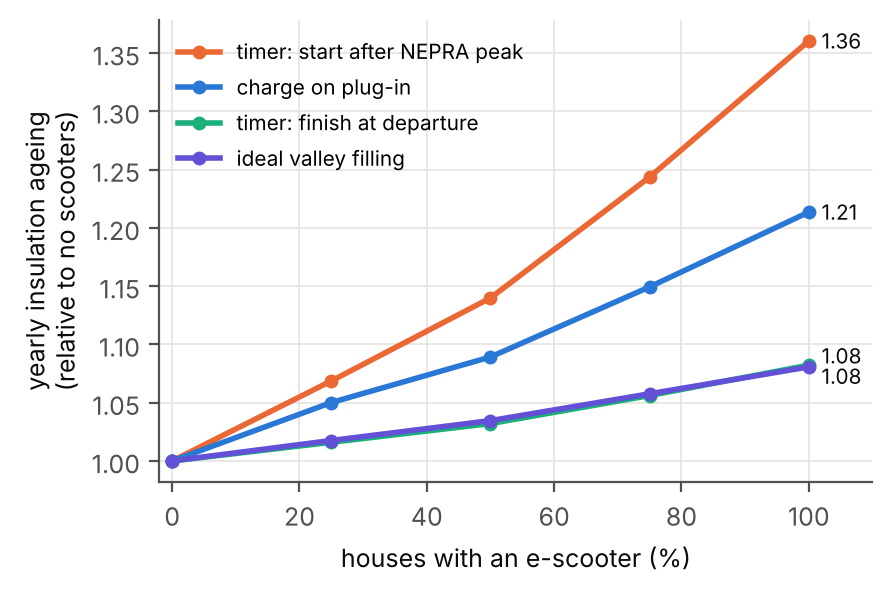
\includegraphics[width=0.76\columnwidth]{f4_adoption.png}
\caption{Yearly insulation ageing against the share of houses with a
scooter, 100~kVA.}
\label{fig:adopt}
\end{figure}

Charging on arrival adds 21\,\%, mostly from delivery riders who plug in at
22:30--23:30, on top of the night peak. The 600~s random delay changes almost
nothing: it spreads starts over minutes, while the transformer responds over
hours. The after-peak timer is the worst rule: it moves commuters from the
early evening to 23:00 and stacks every scooter at one time, so ageing rises
36\,\% and the time above rating goes from 1.7 to 26~h. This is the same
effect that Hilshey \emph{et al.} \cite{hilshey2013} found for an
after-midnight delay of car charging. The ``latest'' rule puts charging in the
early morning, when the load is falling and the air is coolest, and gives the
same yearly ageing as the ideal valley fill. On 75~kVA the order is the same
and the gaps are larger: the after-peak timer doubles ageing and raises the
time above 120\,$^\circ$C from 23.2 to 85.0~h, against 26.7~h for the latest
rule.

\subsection{Sensitivity}
Fig.~\ref{fig:sens} repeats the comparison for other assumptions. The order
after peak $>$ plug-in $>$ latest holds in every case. Delivery riders matter
most: with half of the scooters used for delivery, plug-in charging adds
49\,\%. With only commuters, plug-in adds 8\,\% but the after-peak timer still
adds 24\,\%. With 1~kW chargers the latest rule keeps ageing low but creates a
new morning peak of 1.11~p.u. (07:28 on 5 June), because the delivery
riders' scooters, which share one departure time, start together; real
departure times would spread this. In a few cases the latest rule ages the
transformer slightly less than valley fill (for example 216.9 against
217.2~h with 0.35~kW chargers), because valley fill minimises load and does
not see the ambient temperature. Rooftop PV on 30\,\% of houses lowers
baseline ageing by 20\,\% by cutting the hot afternoon load, but it does not
touch the night peak, so the charging results change little ($+24$\,\%,
$+42$\,\% and $+6$\,\%). This agrees with Behi \emph{et al.} \cite{behi2017},
where PV relieved off-peak loading but not the peak.

\begin{figure}[t]
\centering
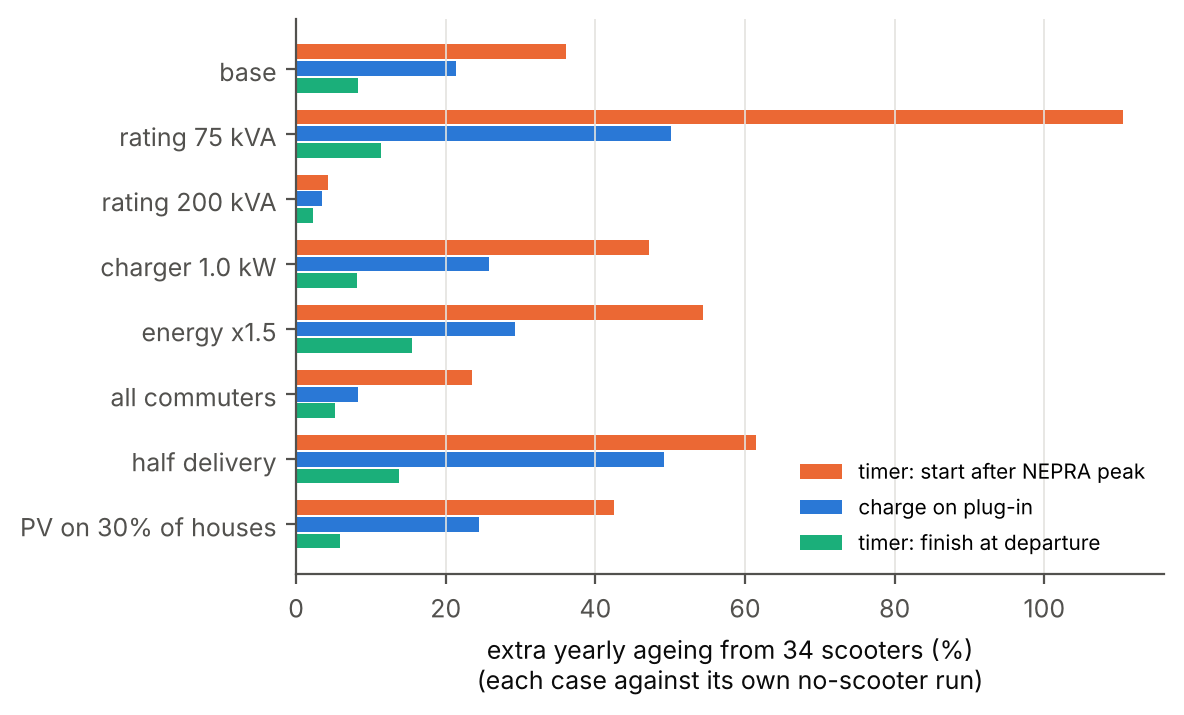
\includegraphics[width=0.78\columnwidth]{f5_sensitivity.png}
\caption{Extra yearly ageing from a scooter in every house under other
assumptions, each against its own no-scooter run.}
\label{fig:sens}
\end{figure}

\subsection{A warmer climate}
Adding 2~K to the air temperature, and to the load through the measured
feeder slope, adds 29.7~MWh (11\,\%) and raises baseline ageing from 200 to
487~h, 2.4 times. This is larger than the effect of any charging rule. With
scooters added in the warmer case, plug-in charging gives 609~h, the
after-peak timer 705~h and the latest rule 526~h. The warming case
extrapolates a one-year relation and should be read as an order of
magnitude, in line with the finding of Hilshey \emph{et al.}
\cite{hilshey2013} that climate can matter as much as the vehicles.

\section{Discussion and Limitations}
The night peak comes straight from the measured data and does not depend on
the transformer model. It changes the practical advice: in such a
neighbourhood ``charge at night after the peak'' is the worst of the simple
rules tested, and ``finish just before you leave'' is as good as the ideal
schedule. A rule like that needs only the departure time and the energy to be
charged, which a scooter charger could ask for.

The limits are real.
\begin{itemize}
\item The 34 houses are not one feeder and are mostly large houses with
several AC units; a real street would differ in size, diversity and mix.
Power factor, the number of houses per transformer and the charger and use
profiles are assumptions, and only the scooter part is a model.
\item Gap-filled minutes were imputed, and load shedding, which the dataset's
authors noted in the records \cite{nadeem2020} and which in reality removes
load in blocks, is not modelled.
\item The train and test weeks alternate, so they share seasons and
neighbouring days are correlated; the test $R^2$ is therefore an optimistic
measure of how the fits would do in another year.
\item Weather is hourly and was interpolated to minutes on the assumption
that each value is the mean of the hour after its time stamp. Air temperature
is used as the transformer's ambient, without sun on the tank.
\item The temperature slope comes from one year and partly reflects seasonal
habits, so the warming case is an extrapolation.
\item The peak windows are from the 2026 tariff, not from 2018--19, and
residential time-of-use applies only to connections with a peak load above
5~kW \cite{nepra2026}.
\end{itemize}

\section{Conclusion}
In one year of measured data from Lahore, household load rises by about 77~W
per kelvin above 22.5\,$^\circ$C, and a 34-house feeder peaks near midnight in
summer. On such a feeder, the time of scooter charging decides its effect on
the transformer more than the energy itself: from $+8$\,\% to $+36$\,\% yearly
ageing for the same 4\,\% more energy. Charging that ends at departure is as
good as the ideal schedule, and charging that starts after the tariff peak is
the worst of the rules tested. A climate 2~K warmer would matter more than
any of them. Natural next steps are measured data from one real feeder,
including load shedding, and a charging rule that also uses the transformer
or air temperature, as proposed for cars in \cite{hilshey2013}.

\section*{Acknowledgment}
The author thanks the Energy Informatics Group at LUMS for publishing PRECON,
and NASA Langley for POWER data. AI-based coding assistance was used for parts
of the software and the first draft of the text; modelling choices, results
and text were checked by the author. Code and data:
\url{https://github.com/tehreem-gillani/lahore-heat-feeder}.

\begin{thebibliography}{99}
\bibitem{saarc2026} SAARC Energy Centre, ``EV charging and the grid,'' training workshop slides, Aug. 2026. [Online]. Available: \url{https://www.saarcenergy.org/wp-content/uploads/2026/08/EV-Charging-and-Grid-ISMO_SAARC.pdf}
\bibitem{pronto} ``New EV scooter Eveon Pronto launched in Pakistan,'' PakWheels Blog, Jan. 2025. [Online]. Available: \url{https://www.pakwheels.com/blog/new-ev-scooter-eveon-pronto-launched-in-pakistan/}
\bibitem{iec60076} \emph{Power transformers -- Part 7: Loading guide for oil-immersed power transformers}, IEC 60076-7:2005.
\bibitem{precon} A. Nadeem and N. Arshad, ``PRECON: Pakistan residential electricity consumption dataset,'' in \emph{Proc. 10th ACM Int. Conf. Future Energy Systems (e-Energy '19)}, Phoenix, AZ, USA, 2019, pp. 52--57, doi: 10.1145/3307772.3328317.
\bibitem{nasapower} NASA Langley Research Center, ``Prediction of Worldwide Energy Resources (POWER) project, hourly API,'' [Online]. Available: \url{https://power.larc.nasa.gov}, accessed Oct. 2026.
\bibitem{gillaniA} S. T. Gillani, ``Look-ahead battery reserve for rooftop PV under scheduled load-shedding: A perfect-foresight benchmark study for Karachi,'' code and results, GitHub repository, 2026. [Online]. Available: \url{https://github.com/tehreem-gillani/pv-battery-ems-karachi}
\bibitem{gillani2} S. T. Gillani, ``Climate or design? Mission-profile thermal cycling of electric two-wheeler motor controllers in five cities,'' technical report, 2026. [Online]. Available: \url{https://github.com/tehreem-gillani/e2w-controller-wearout}
\bibitem{gong2012} Q. Gong, S. Midlam-Mohler, V. Marano, and G. Rizzoni, ``Study of PEV charging on residential distribution transformer life,'' \emph{IEEE Trans. Smart Grid}, vol. 3, no. 1, pp. 404--412, 2012, doi: 10.1109/TSG.2011.2163650.
\bibitem{hilshey2013} A. D. Hilshey, P. D. H. Hines, P. Rezaei, and J. R. Dowds, ``Estimating the impact of electric vehicle smart charging on distribution transformer aging,'' \emph{IEEE Trans. Smart Grid}, vol. 4, no. 2, pp. 905--913, 2013, doi: 10.1109/TSG.2012.2217385.
\bibitem{soleimani2020} M. Soleimani and M. Kezunovic, ``Mitigating transformer loss of life and reducing the hazard of failure by the smart EV charging,'' \emph{IEEE Trans. Ind. Appl.}, vol. 56, no. 5, pp. 5974--5983, 2020, doi: 10.1109/TIA.2020.2986990.
\bibitem{clementnyns2010} K. Clement-Nyns, E. Haesen, and J. Driesen, ``The impact of charging plug-in hybrid electric vehicles on a residential distribution grid,'' \emph{IEEE Trans. Power Syst.}, vol. 25, no. 1, pp. 371--380, 2010, doi: 10.1109/TPWRS.2009.2036481.
\bibitem{geiles2013} T. Geiles and S. Islam, ``Impact of PEV charging and rooftop PV penetration on distribution transformer life,'' in \emph{Proc. IEEE PES General Meeting}, 2013, pp. 1--5, doi: 10.1109/PESMG.2013.6672211.
\bibitem{behi2017} B. Behi, A. Arefi, H. Pezeshki, and F. Shahnia, ``Distribution transformer lifetime analysis in the presence of demand response and rooftop PV integration,'' \emph{Renew. Energy Environ. Sustain.}, vol. 2, art. 27, 2017, doi: 10.1051/rees/2017013.
\bibitem{muratori2018} M. Muratori, ``Impact of uncoordinated plug-in electric vehicle charging on residential power demand,'' \emph{Nature Energy}, vol. 3, no. 3, pp. 193--201, 2018, doi: 10.1038/s41560-017-0074-z.
\bibitem{powell2022} S. Powell, G. V. Cezar, L. Min, I. M. L. Azevedo, and R. Rajagopal, ``Charging infrastructure access and operation to reduce the grid impacts of deep electric vehicle adoption,'' \emph{Nature Energy}, vol. 7, no. 10, pp. 932--945, 2022, doi: 10.1038/s41560-022-01105-7.
\bibitem{lijenn2024} Y. Li and A. Jenn, ``Impact of electric vehicle charging demand on power distribution grid congestion,'' \emph{Proc. Natl. Acad. Sci. USA}, vol. 121, no. 18, art. e2317599121, 2024, doi: 10.1073/pnas.2317599121.
\bibitem{auffhammer2017} M. Auffhammer, P. Baylis, and C. H. Hausman, ``Climate change is projected to have severe impacts on the frequency and intensity of peak electricity demand across the United States,'' \emph{Proc. Natl. Acad. Sci. USA}, vol. 114, no. 8, pp. 1886--1891, 2017, doi: 10.1073/pnas.1613193114.
\bibitem{kissock2003} J. K. Kissock, J. S. Haberl, and D. E. Claridge, ``Inverse modeling toolkit: Numerical algorithms,'' \emph{ASHRAE Trans.}, vol. 109, no. 2, 2003.
\bibitem{nadeem2020} A. Nadeem and N. Arshad, ``Short term load forecasting on PRECON dataset,'' in \emph{Proc. Int. Conf. Advances in the Emerging Computing Technologies (AECT)}, 2020, pp. 1--6, doi: 10.1109/AECT47998.2020.9194176.
\bibitem{bajwa2026} M. N. Bajwa, M. A. Jamil, H. Yaqoob, M. W. Shahzad, and M. M. Fraz, ``Multi-city analysis of climate trends, cooling demand, and residential electricity use in Pakistan,'' \emph{Energy Convers. Manag.: X}, vol. 31, art. 102203, 2026, doi: 10.1016/j.ecmx.2026.102203.
\bibitem{abdulmanan2022} A. F. N. Abdul-Manan \emph{et al.}, ``Electrifying passenger road transport in India requires near-term electricity grid decarbonisation,'' \emph{Nature Commun.}, vol. 13, art. 2095, 2022, doi: 10.1038/s41467-022-29620-x.
\bibitem{corti2024} F. Corti, S. D. Iacono, D. Astolfi, M. Pasetti, A. Vasile, A. Reatti, and A. Flammini, ``A comprehensive review of charging infrastructure for electric micromobility vehicles: Technologies and challenges,'' \emph{Energy Rep.}, vol. 12, pp. 545--567, 2024, doi: 10.1016/j.egyr.2024.06.026.
\bibitem{huu2021} D. N. Huu and V. N. Ngoc, ``A two-level desired load profile tracking algorithm for electric two-wheeler charging stations,'' \emph{Eng. Technol. Appl. Sci. Res.}, vol. 11, no. 6, pp. 7814--7823, 2021, doi: 10.48084/etasr.4552.
\bibitem{ukscp} \emph{The Electric Vehicles (Smart Charge Points) Regulations 2021}, UK Statutory Instrument 2021 No. 1467.
\bibitem{nepra2026} National Electric Power Regulatory Authority, ``Determination of tariff for LESCO in light of revised annual rebasing timelines,'' TRF-603 \& TRF-604, 7 Jan. 2026, schedule of tariff, cl.~10.
\bibitem{is2026} Bureau of Indian Standards, IS 2026 (Part 7):2009, identical with IEC 60076-7:2005. [Online]. Available: \url{https://law.resource.org/pub/in/bis/S05/is.2026.7.2009.pdf}
\end{thebibliography}

\end{document}
